%
% introduction
\section{Client}
\label{sec:software-coral-intro}
The software that acts as a client on the Coral dev-board, presented in chapter
(\ref{sec:hard-devboard}), created by Google is based on the same Qt framework previously
introduced in order to guarantee portability and reliability of the code. This,
remember, has an ARM Cortex-A53 processor, but unlike the one mounted on
Raspberry it executes 64-bit code and takes advantage of the new \textbf{armv8a}
architecture with a significant performance gain. This difference arises from
the execution of Machine Learning operations supported by the TPU, described in
detail in section (\ref{sec:hard-tpu}).
%
% interface
As seen for the main program, here too we find a main interface executed in the
main thread. The simplest interface is divided into two areas: the first one
where it is possible to observe the flow of images coming from the TCP socket.
As hows in figure (\ref{fig:software-socket-server-client}).\hfill \break
On the other hand, the second zone offers the possibility of
connecting to the TCP socket by entering the address and port of the machine on
which the server is run, which is listening for possible connection requests.
Once the connection between the server and the client is established, the label
is updated with the images received. 
%
%
\begin{figure}[htb]
	\centering
	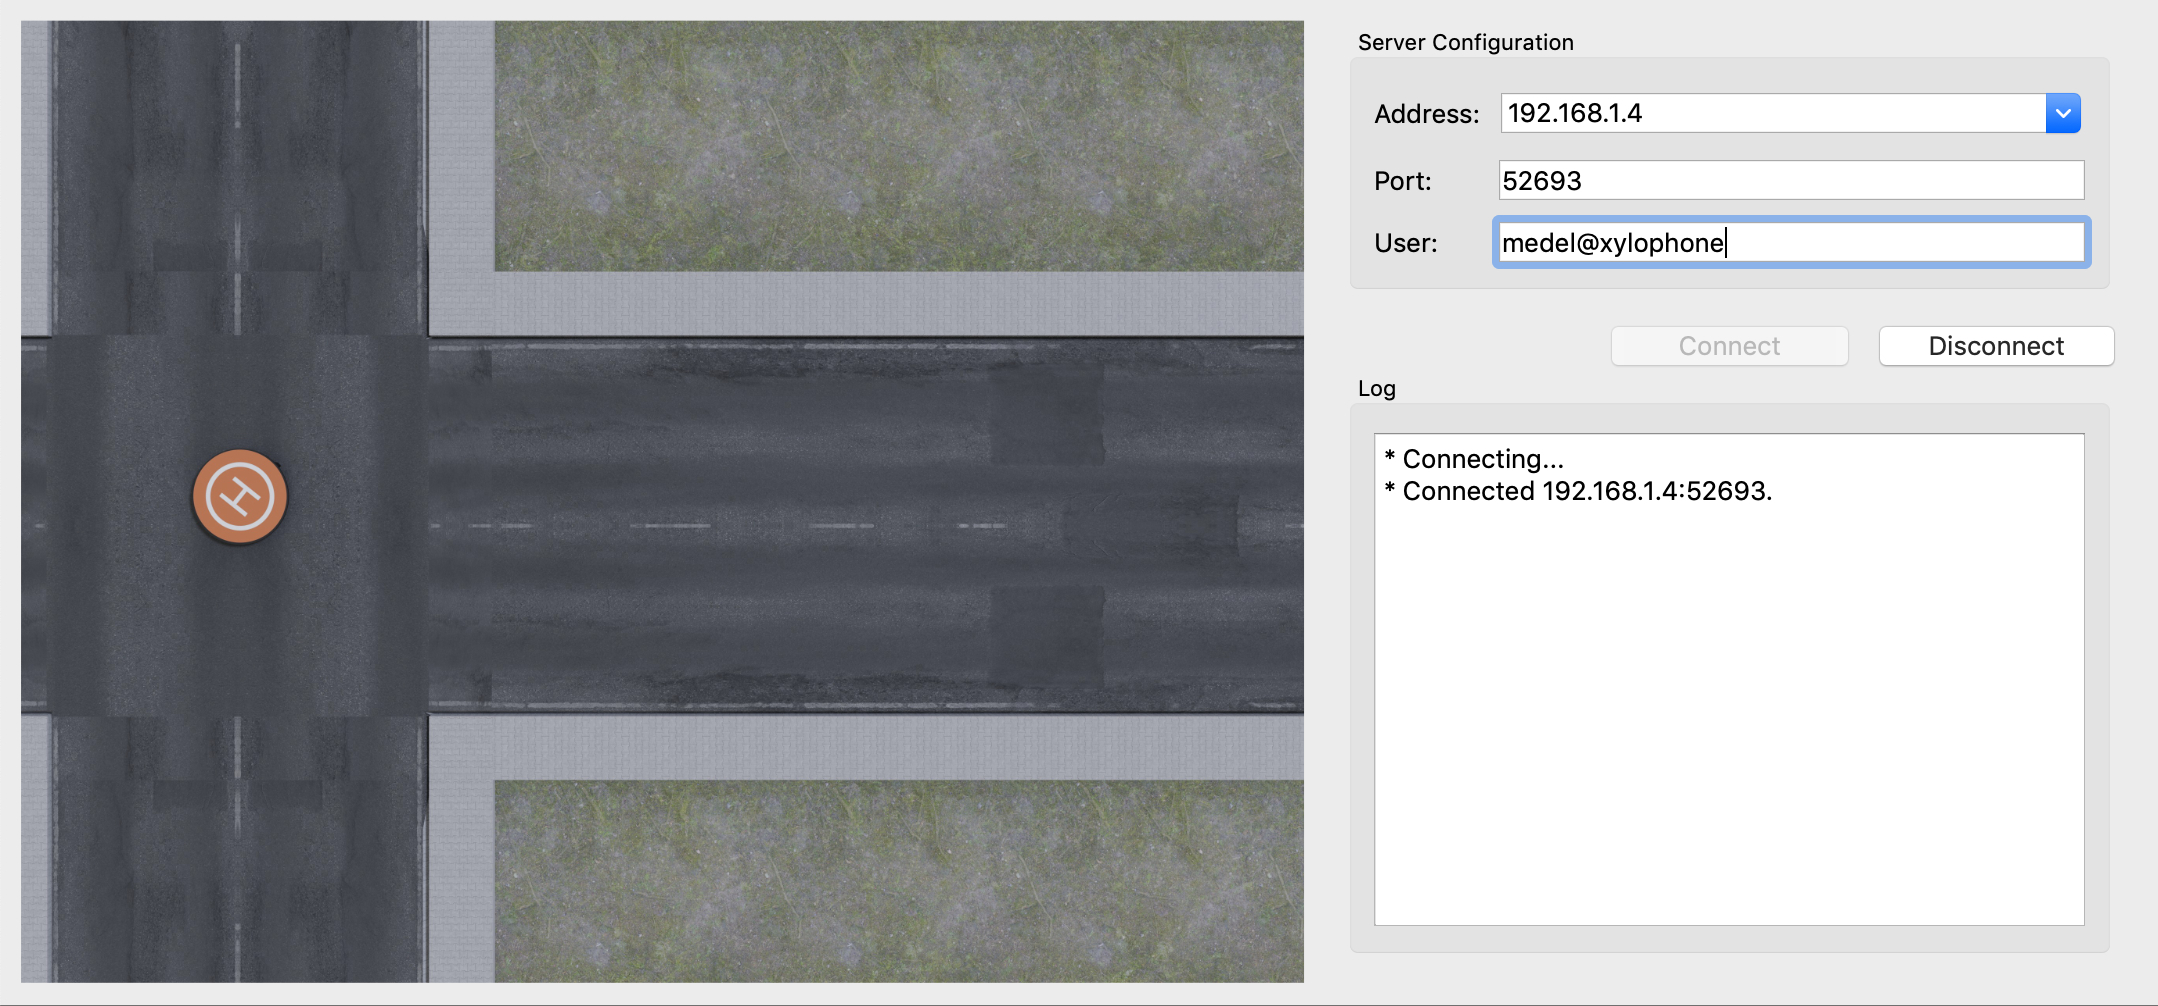
\includegraphics[width=0.7\textwidth]{client_ui.jpg}
	\caption{User interface client application.}
	\label{fig:software-client-ui}
\end{figure}
%
% software analysis
\subsection{Software Analysis}
\label{ssec:software-coral-analysis}
To avoid blockages and unpleasant delays in receiving images from the TCP
socket, multi-thread programming was used. In fact, as previously described, the
interface managed by QWidget is run on the main thread. If the connection is
stable, the thread starts which allows reception in a queue waiting to leave.\\ 
On the other hand, this is prepared when the class is instantiated within the
main function. Since this infinite cycle is the critical factor, we analyse its
structure in detail below.
%
% code list
\begin{listing}[ht] 
\inputminted[frame=lines,framesep=2mm, linenos=true, autogobble, breaklines=true, fontsize=\scriptsize, firstline=12, lastline=26]{c++}{software/code/streamerthread.cpp} 
\caption{Particular report function sending image.} 
\label{lst:coral-client-code} 
\end{listing}
%
\\As you can see in the function code, shown in Listing
(\ref{lst:coral-client-code}), we observe the instance of the \texttt{socket}
member object of the \texttt{QTcpSocket} class type. 
By starting the connection, the server starts to transmit the frame. 
The critical section from the \emph{while loop} is protected by a mutex,
highlighted by the \texttt{QMutexLocker} class, a mutex indicates a
process of synchronization between concurrent processes or threads, with which
multiple parallel tasks are prevented from simultaneously accessing 
data in memory or other resources subject to race condition.\cite{wiki:mutex} \hfill \break
Locking and unlocking a \texttt{QMutex} in complex functions and statements or
in exception handling code is error-prone.
\texttt{QMutexLocker} can be used in such situations to ensure that the state of the
mutex is always well-defined. \texttt{QMutexLocker} should be created within a
function where a \texttt{QMutex} needs to be locked. The mutex is locked when
\texttt{QMutexLocker} is created. If locked, the mutex will be unlocked when
the \texttt{QMutexLocker} is destroyed.
Using \texttt{QMutexLocker} greatly simplifies the code, and makes it more
readable.\cite{Qt:QMutexclass}\\
\\\noindent The buffer is filled with reading from the socket and before putting the signal
to update the image in the interface a small interval of time is waited to
guarantee the complete reception of the image.
Before updating the label on the dashboard, filter the image to verify that it
is consistent and different from an empty or corrupt image, shown in listing
(\ref{lst:coral-ui-code}). 
If this occurs, the function is immediately exited to
avoid viewing an image being ready to receive a new image. 
%
% code list
\begin{listing}[ht] 
\inputminted[frame=lines,framesep=2mm, linenos=true, autogobble, breaklines=true, fontsize=\scriptsize, firstline=88, lastline=100]{c++}{software/code/tcpclient.cpp} 
\caption{Implementation filter for empty JPEG image.} 
\label{lst:coral-ui-code} 
\end{listing}
